\section{Domain Analysis}

\graphicspath{ {./Images/} }

\subsection{Impact of the problem over the domain of study}
\par Is there anything more symbolic of the absurdity of modern life than how hard it is to make plans with friends? 

First, you must decide how to get in touch. Email? It's fine, but then you have to deal with 20 replies. Apps like WhatsApp or Signal rarely work because not everyone is on them. And relying only on Facebook guarantees you miss those friends who no longer — or never did — have an account. In short, it's a mess before you even get started. 

Then there is the almost comical back and forth of trying to find a time and day that works for everyone in our busy, scattered lives. Meetings, soccer practices, vacations, tickets to see a show, babysitting dilemmas — they are all part of an endless litany of stuff we fill our days with. It's a wonder we see our friends at all. 

Sure, it's great fodder for standup comedians, but it's also sort of maddening: As digital tech has made many basic things like communicating, shopping, or ordering food more convenient, getting some pals together for drinks is apparently beyond us. 

The problem? The calendar app is broken and sorely in need of reinvention. 

ADVERTISEMENT 

Consider how the calendar compares to email. Though they both started as "professional" tools, now essentially everyone who has access to the internet has an email account. The same cannot be said for calendars. That is an indictment of modern calendar apps all on its own. Sure, some of your nerdy friends send you a Google Calendar invite, but most wouldn't think to. 

To explain why calendar apps are so bad, it helps to think about their roots. While scheduling applications were included with Windows and on the Macintosh from early on, they didn't really take off until the arrival of the internet. In the corporate world, it was Microsoft Exchange and Outlook that came to dominate, and in many cases, still do; even now, 70 percent of Fortune 500 companies rely on Microsoft software. 

But those corporate roots are also why calendar apps are so clunky. For people on the same system, features gradually expanded to include things like setting up meetings, showing yourself as busy, and more. Yet, it also meant that while anyone with an email address could send a message to anyone else with one, calendars remained cordoned off. Now, despite efforts to develop universal standards for calendars, nothing has really taken hold. There are at least three or four choices, instead of just a single universal one. 

Yes, fine, this all sounds a bit arcane, and it is. But that's just the problem. Regular people need calendars, too. Imagine how much easier the basic act of getting people together or organizing your family's time would be if everyone could simply propose times for an event and have other people sign on or not, or have a fast, clean, shared calendar that everyone can see and edit quickly. Right now, because there is no universal standard, that is either impossible or needlessly difficult. 

What needs to change? First, the digital calendar needs to become more like email: Everyone should be able to have one, and regardless of what app you use, all the basic functions — you know, proposing or listing a place, blocking off time to prevent overlap, invite lists, and so on — should all be standard. It shouldn't matter if you were on a Mac or on Microsoft's Outlook or in Google Calendar. It should just work. 

To talk of a calendar app as the solution to our social woes is perhaps to miss the bigger picture: If our lives weren't both so regimented and segmented, perhaps an app to carve out one's time into chunks might not be necessary. And that's to say nothing of the competitive market forces that would get in the way of making the calendar better: Facebook wants its calendar not to work with others so you stay on its platform, and Microsoft, Google, and others are no different. 

But it's for this reason why it's important to push for a reinvention of the calendar app. The web and digital tools are at their most useful and equitable when they are predicated on standards — when they allow whoever wants to use them to do so, without restriction, and without the coercion of making everyone use the same tool. 



We decided to go with this project idea due to the sheer amount of learning possibilities it offers – the main requirement would be a better understanding of OOP/PO/CRUD concepts, as they will be main way of building our codebase for the project.  

The usage of sessions and relational data-bases for storing session and user related information which has a steep learning curve but is well worth the investment as it is a fundamental practice in building todays web services and application. 

And finally, the backend and technology stack used for delivering the project – this requires a good understanding of CI/CD practices as well as different frameworks and a good knowledge of the server-side part and how things work over the network (GET/POST/HTTPS requests, etc...) 
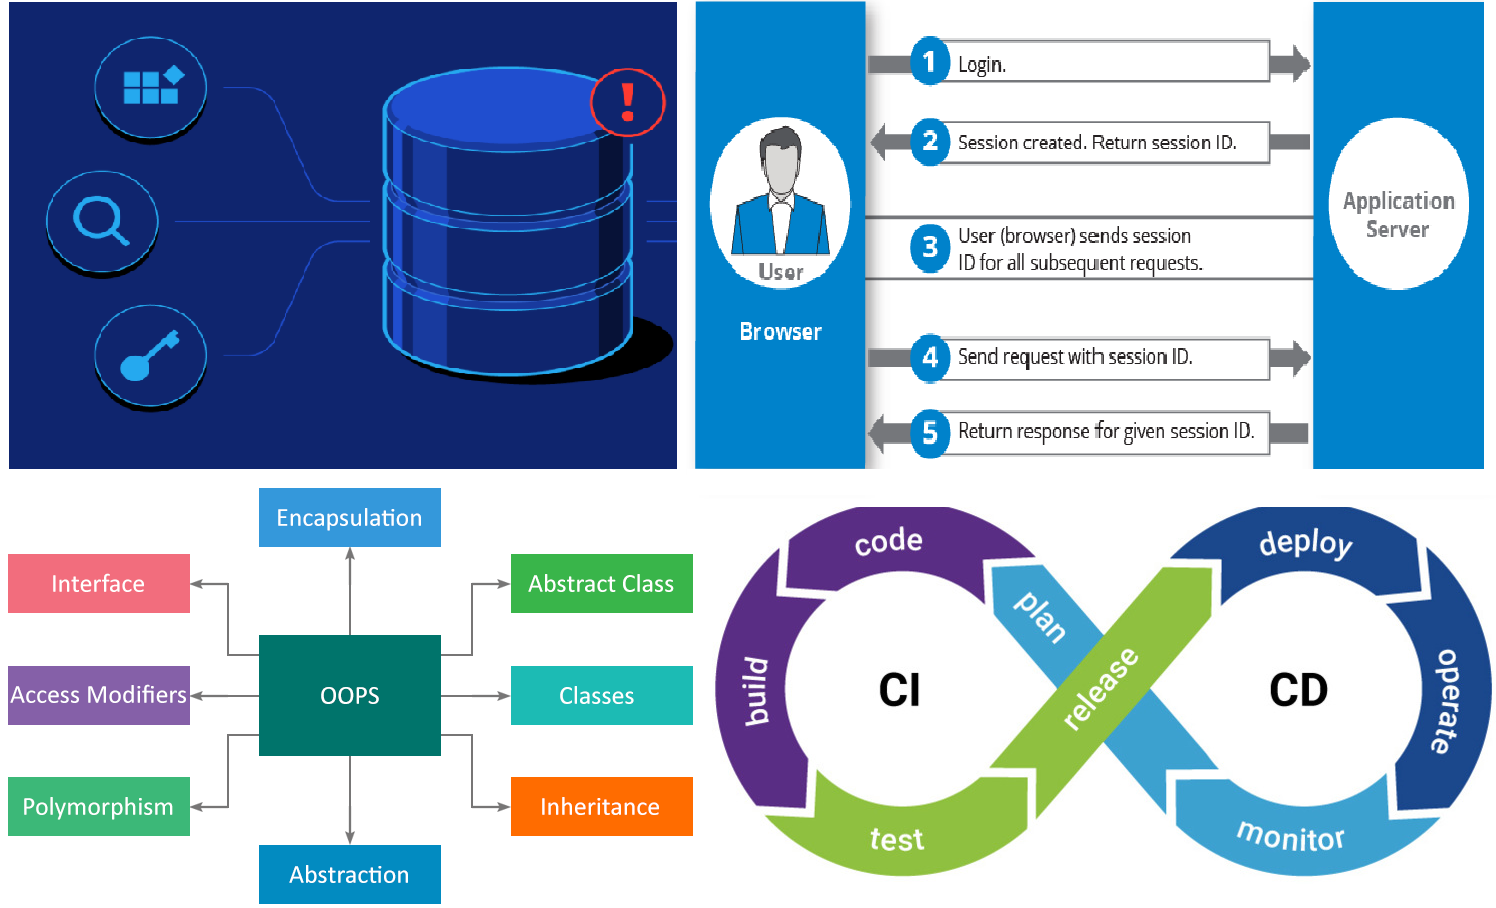
\includegraphics[width=\textwidth]{fotka1}

\subsection{Target group}
\par In order to start working we check the amount of people that are using digital calendars which we took results from ECAL annual survey aimed on aged between 18-64 years from all geographical locations across Australia. The results are that 70\% rely on digital calendars. 
\par 
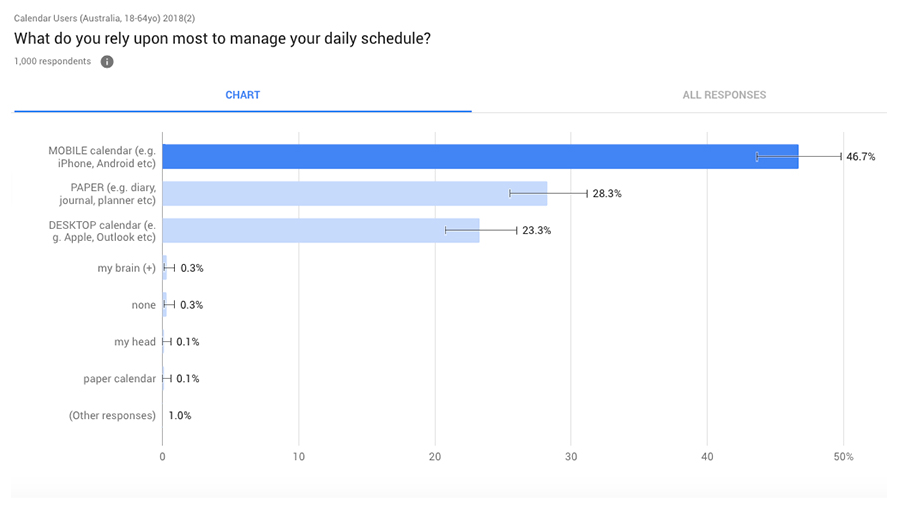
\includegraphics[width=\textwidth]{General_CalendarUsage_Statistic}
\par To understand the target group and customer interest in such a product, we conducted our own survey in which 58 persons took part. This survey helped us to understand to which age group, gender and occupation future customers will identify.    
\par
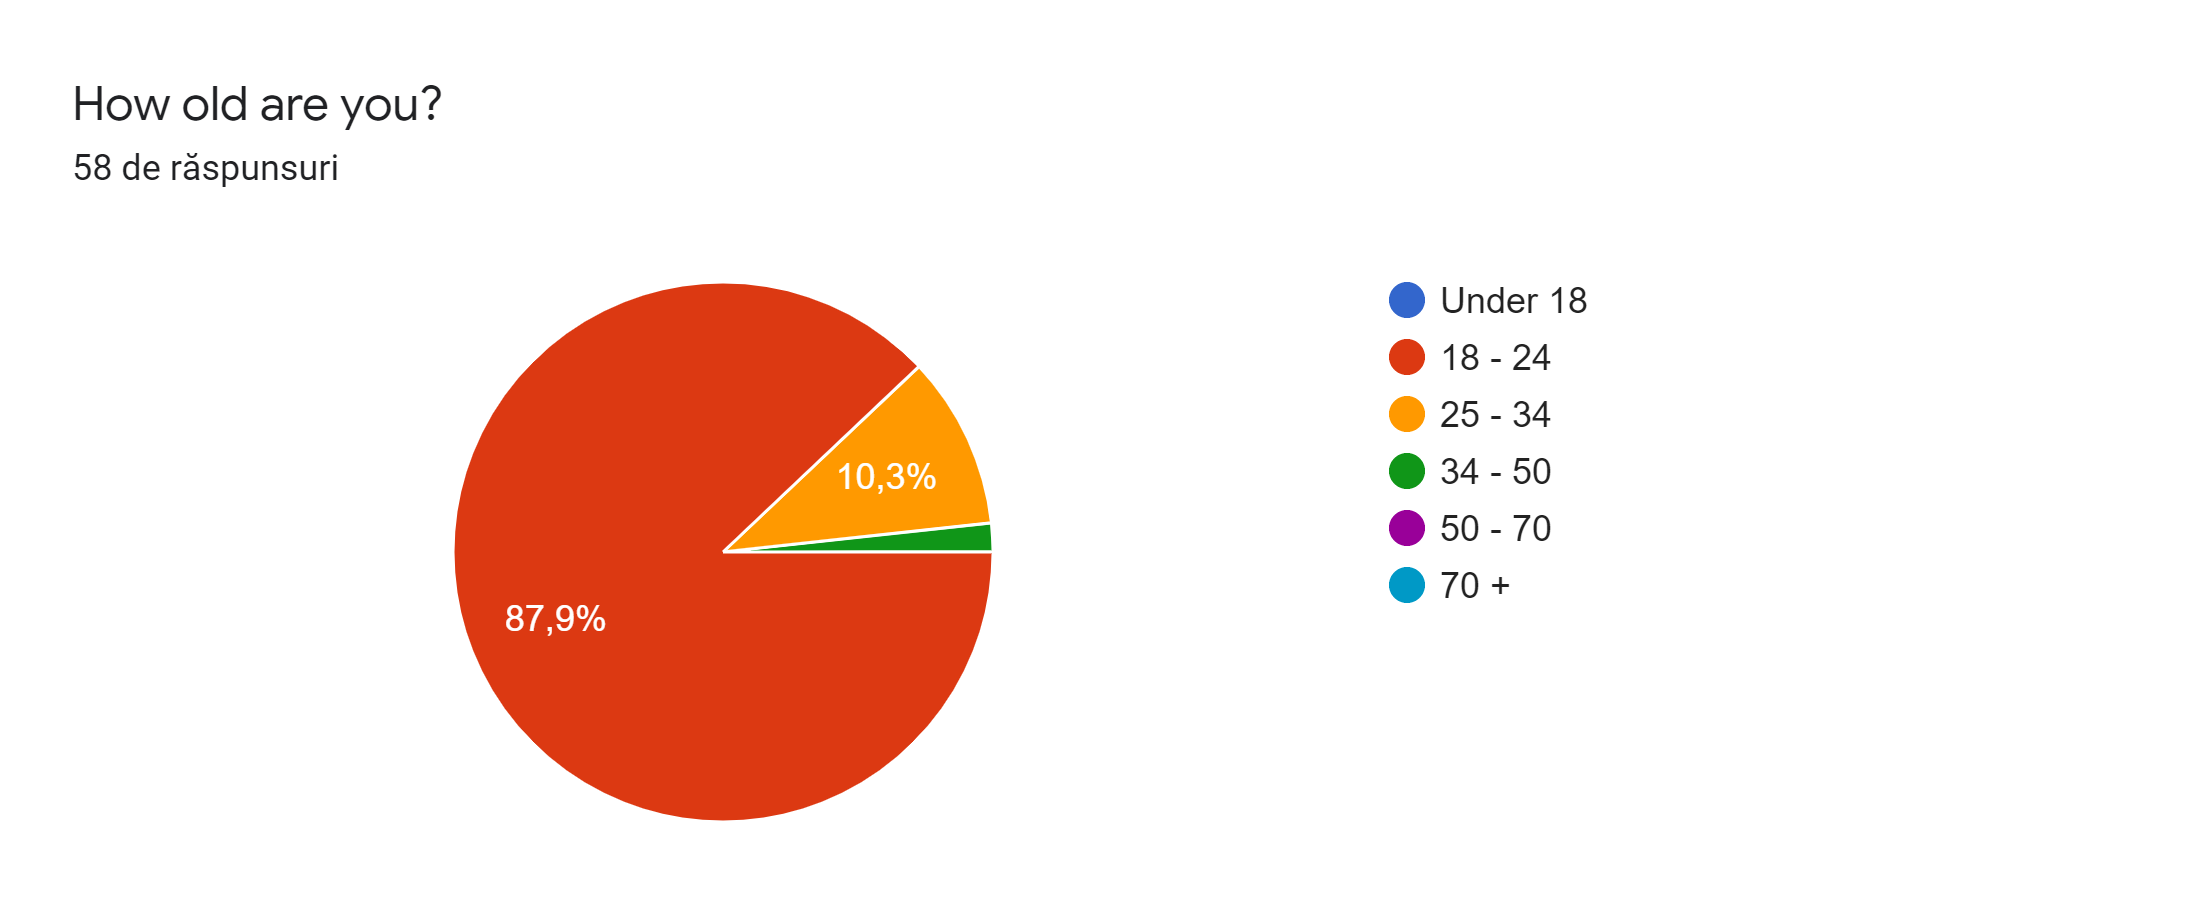
\includegraphics[width=\textwidth]{TargetGroup1}
\par
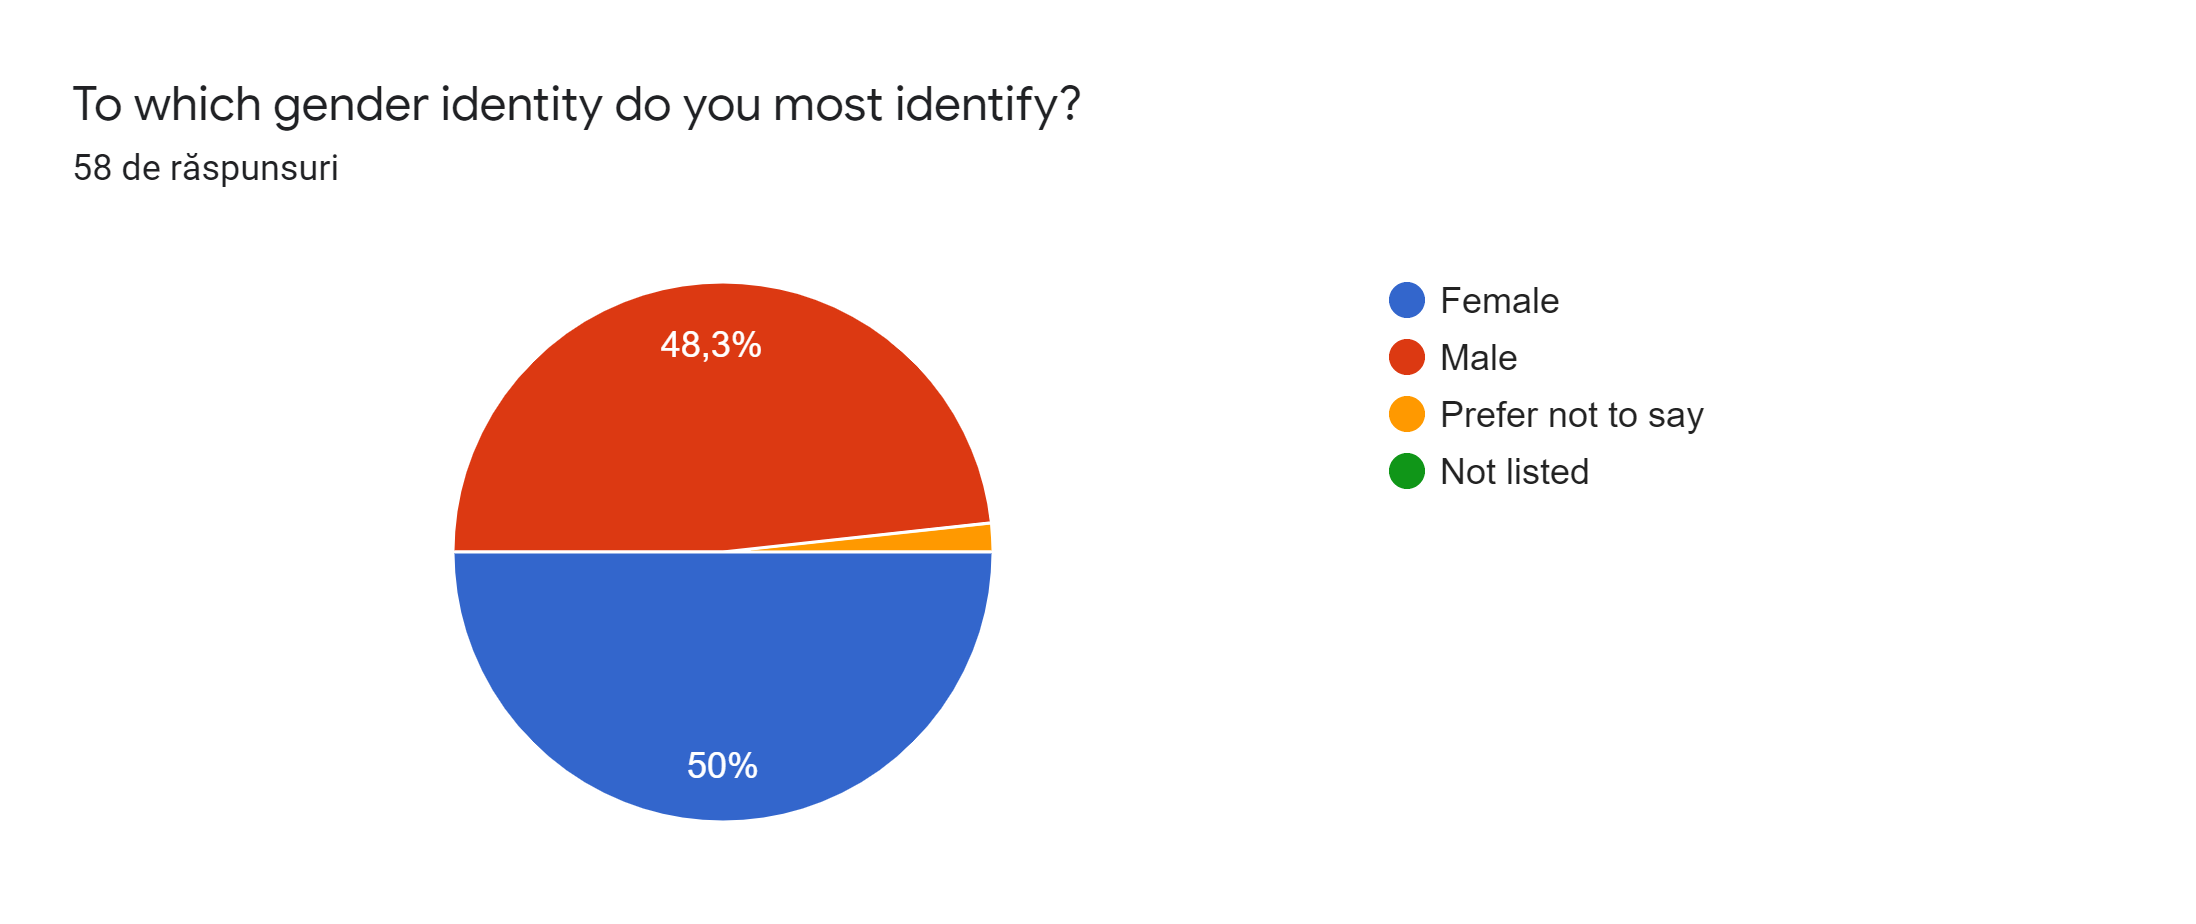
\includegraphics[width=\textwidth]{TargetGroup2}
\par The main advantage of this survey that gender majorities are in equal parts and we have a fair opinion about our product. 
\par
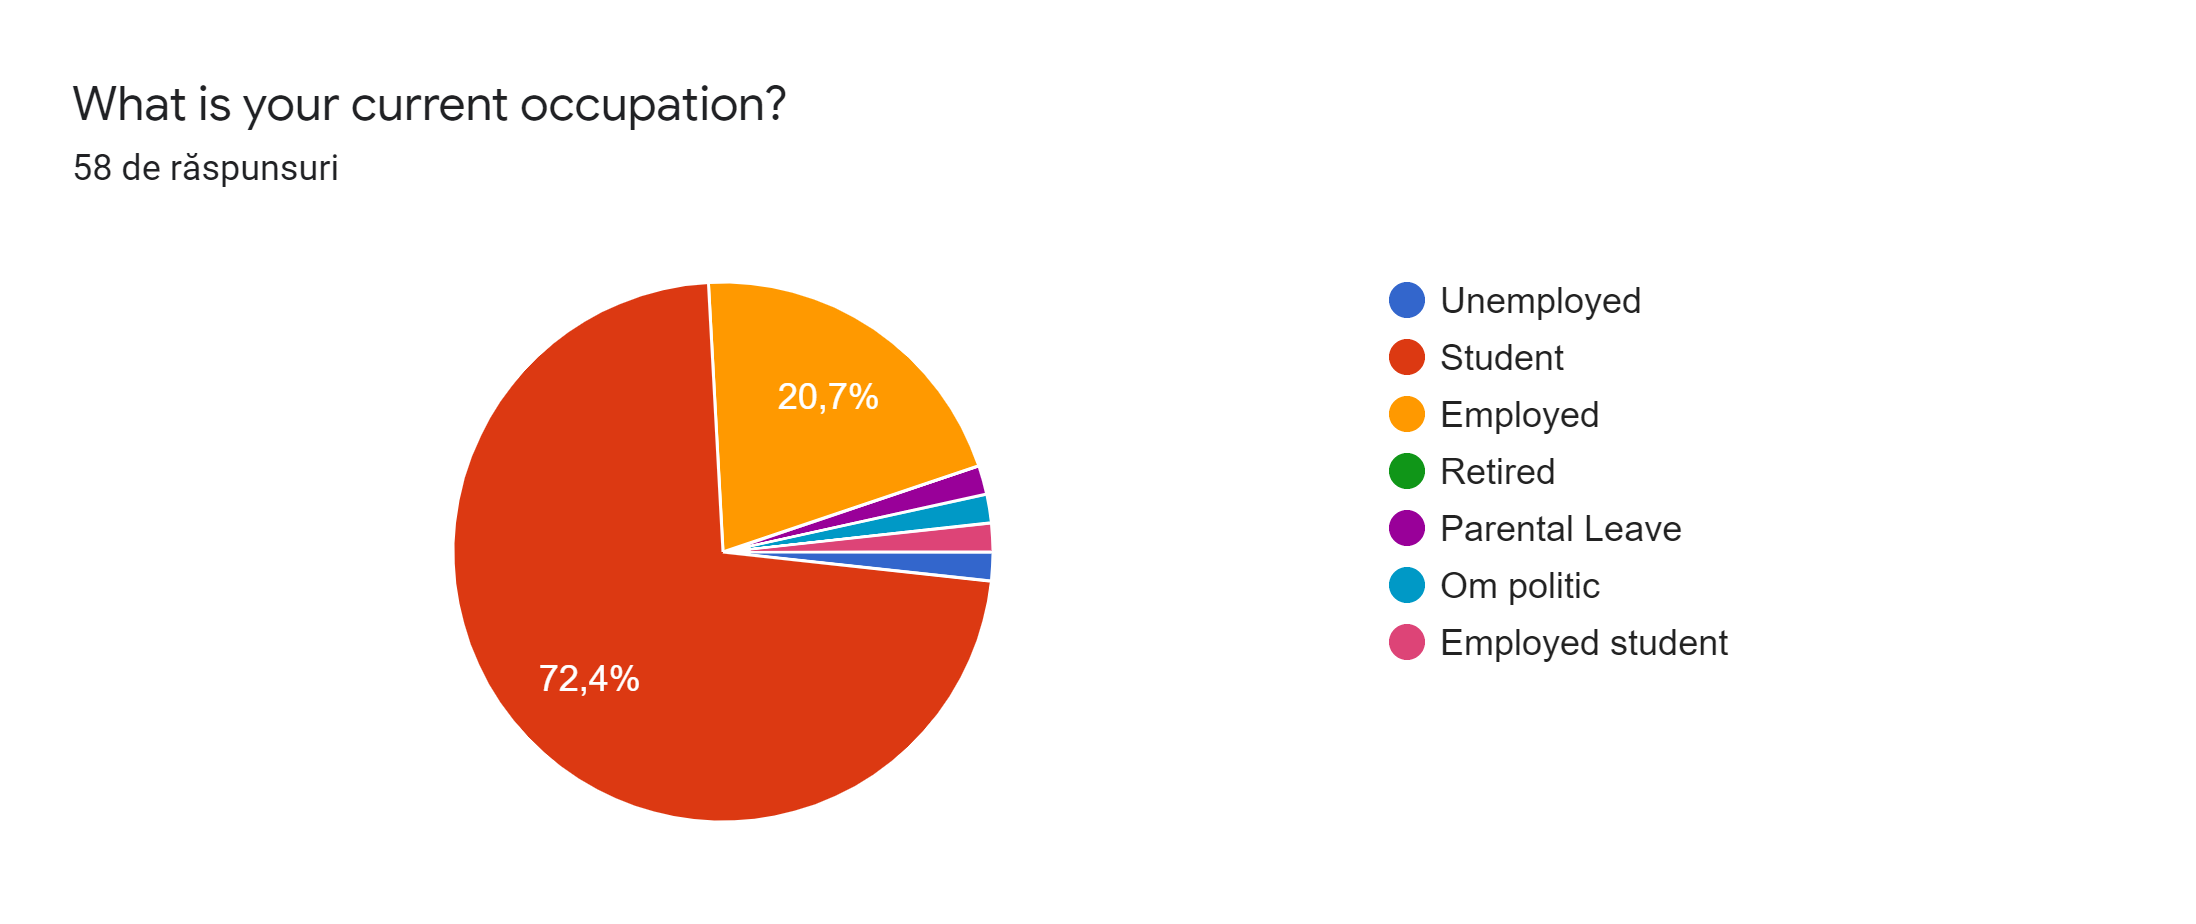
\includegraphics[width=\textwidth]{TargetGroup3}
\par Here we can see that the main parts of audience will be students and employed people. At the end of survey, we had the input line for suggestions, ideas and someone that took part in survey had written to add one more field with employed student. We thought that better will be to add ‘others’ field such that people will have more freedom to describe their current occupation. This way, we have politicians here. 
After these 3 questions we understood that the leading audience of the app will be English speaking active study-working people aged between 16 and 35 which have a lot of tasks events which are related to teams or companies that work on different platforms, or for startuppers who have an extremely flexible schedule and need a platform which will help to organize all tasks and events on one board. 


\subsection{Customer validation}
\par Another part of survey had the aim to find out if people are interested in such an app or not. Firstly, we had to find out which are their habits about organization and time management. 
\par
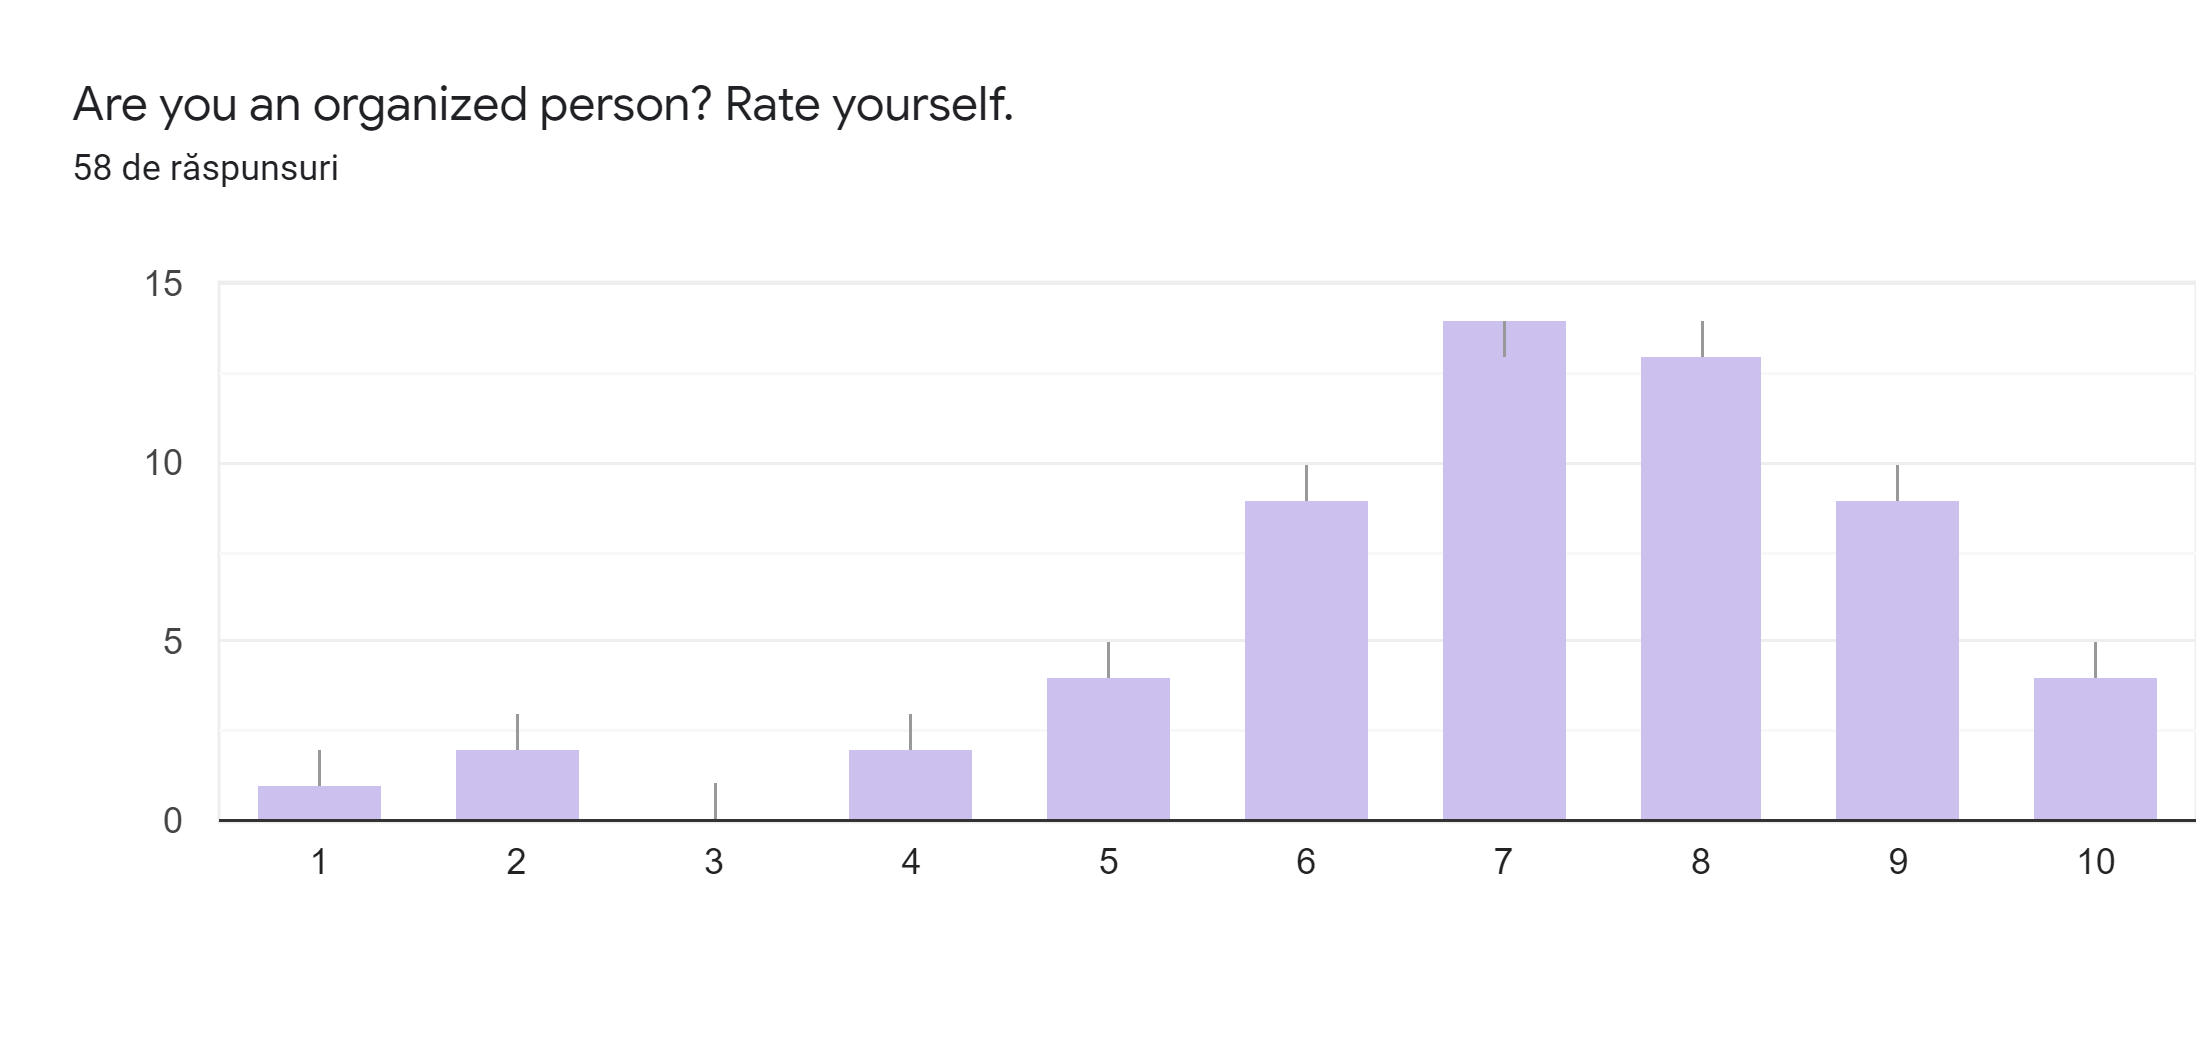
\includegraphics[width=\textwidth]{CustomerValidation1}
\par As we can see most people consider themselves moderately organized, because more than 25 people grade themselves with and 7 or 8. So we understand that people are not enough satisfied of their coordination.
\par
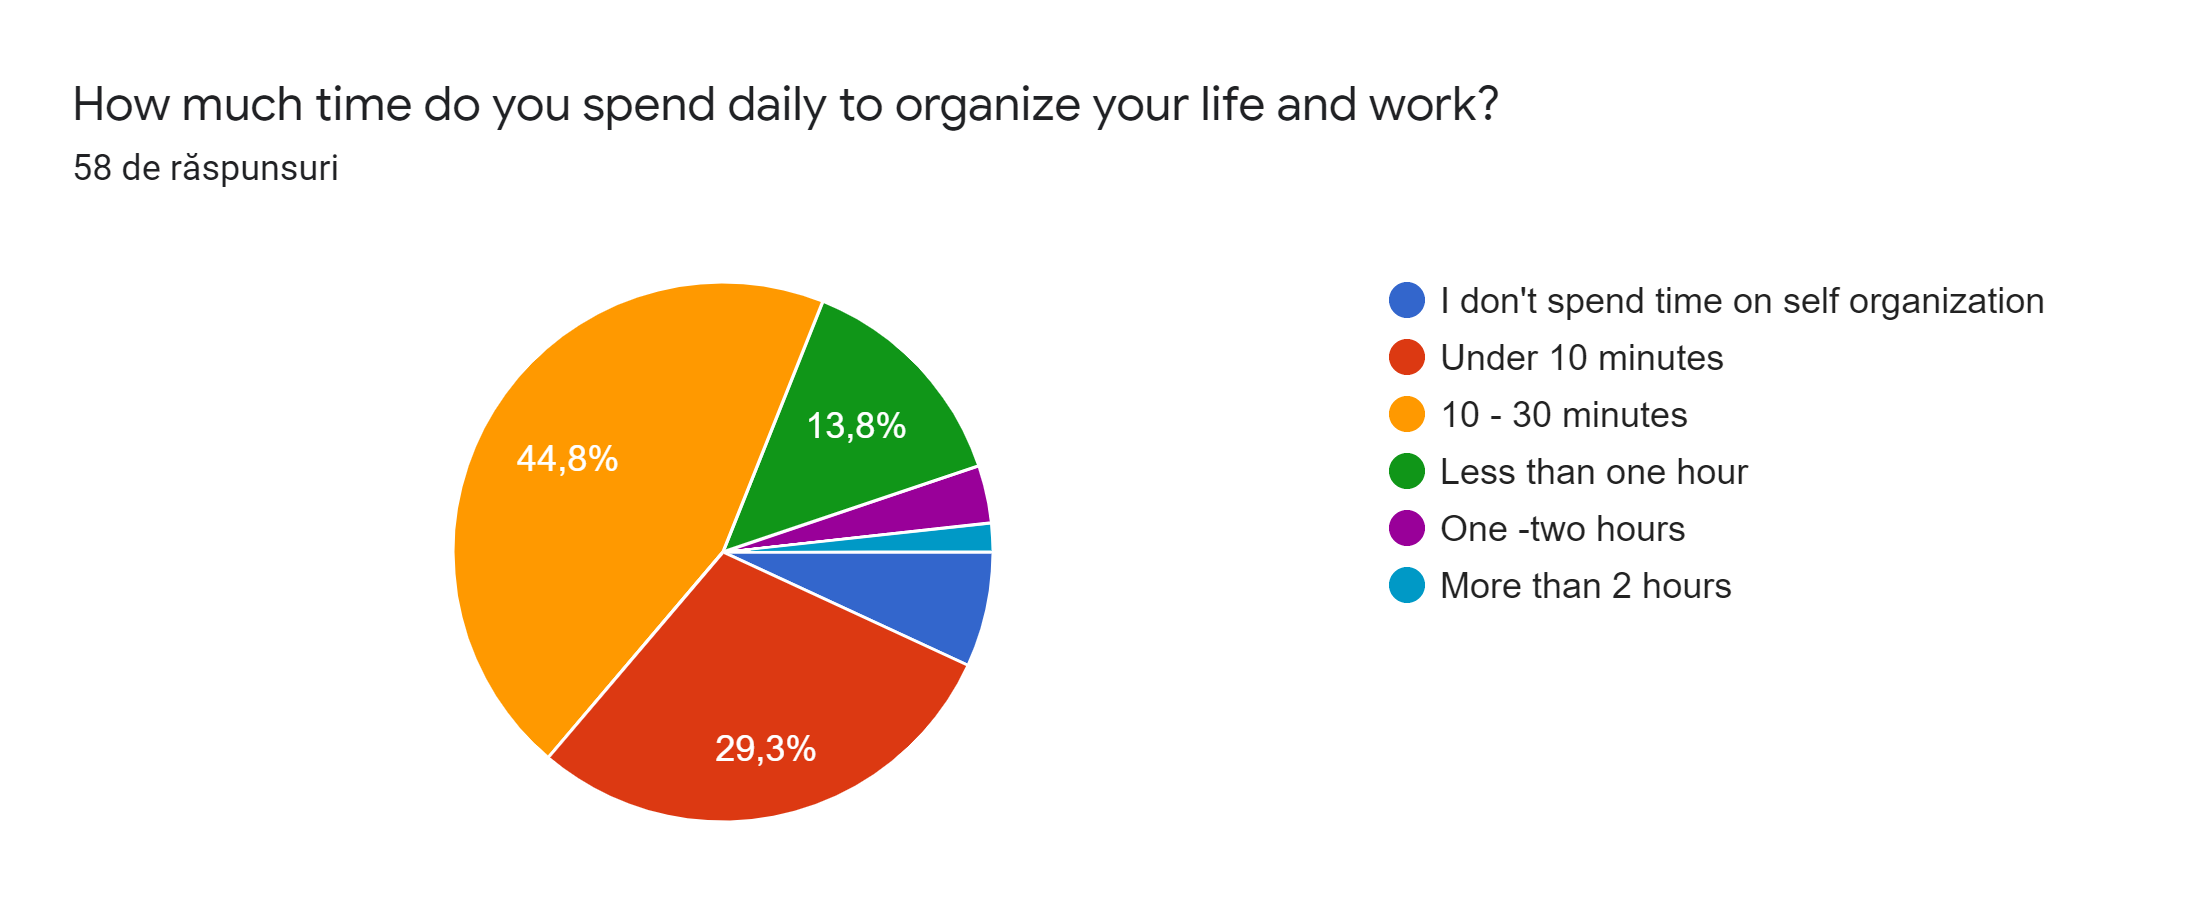
\includegraphics[width=\textwidth]{CustomerValidation2}
\par 44,8 \% of people spend 10-30 minutes per day to plan their life and work. Per year they spend 7300 minutes on this. It is 121 hours, 5 days. In their entire life they spend 250 days on arranging. There is a lot.
\par
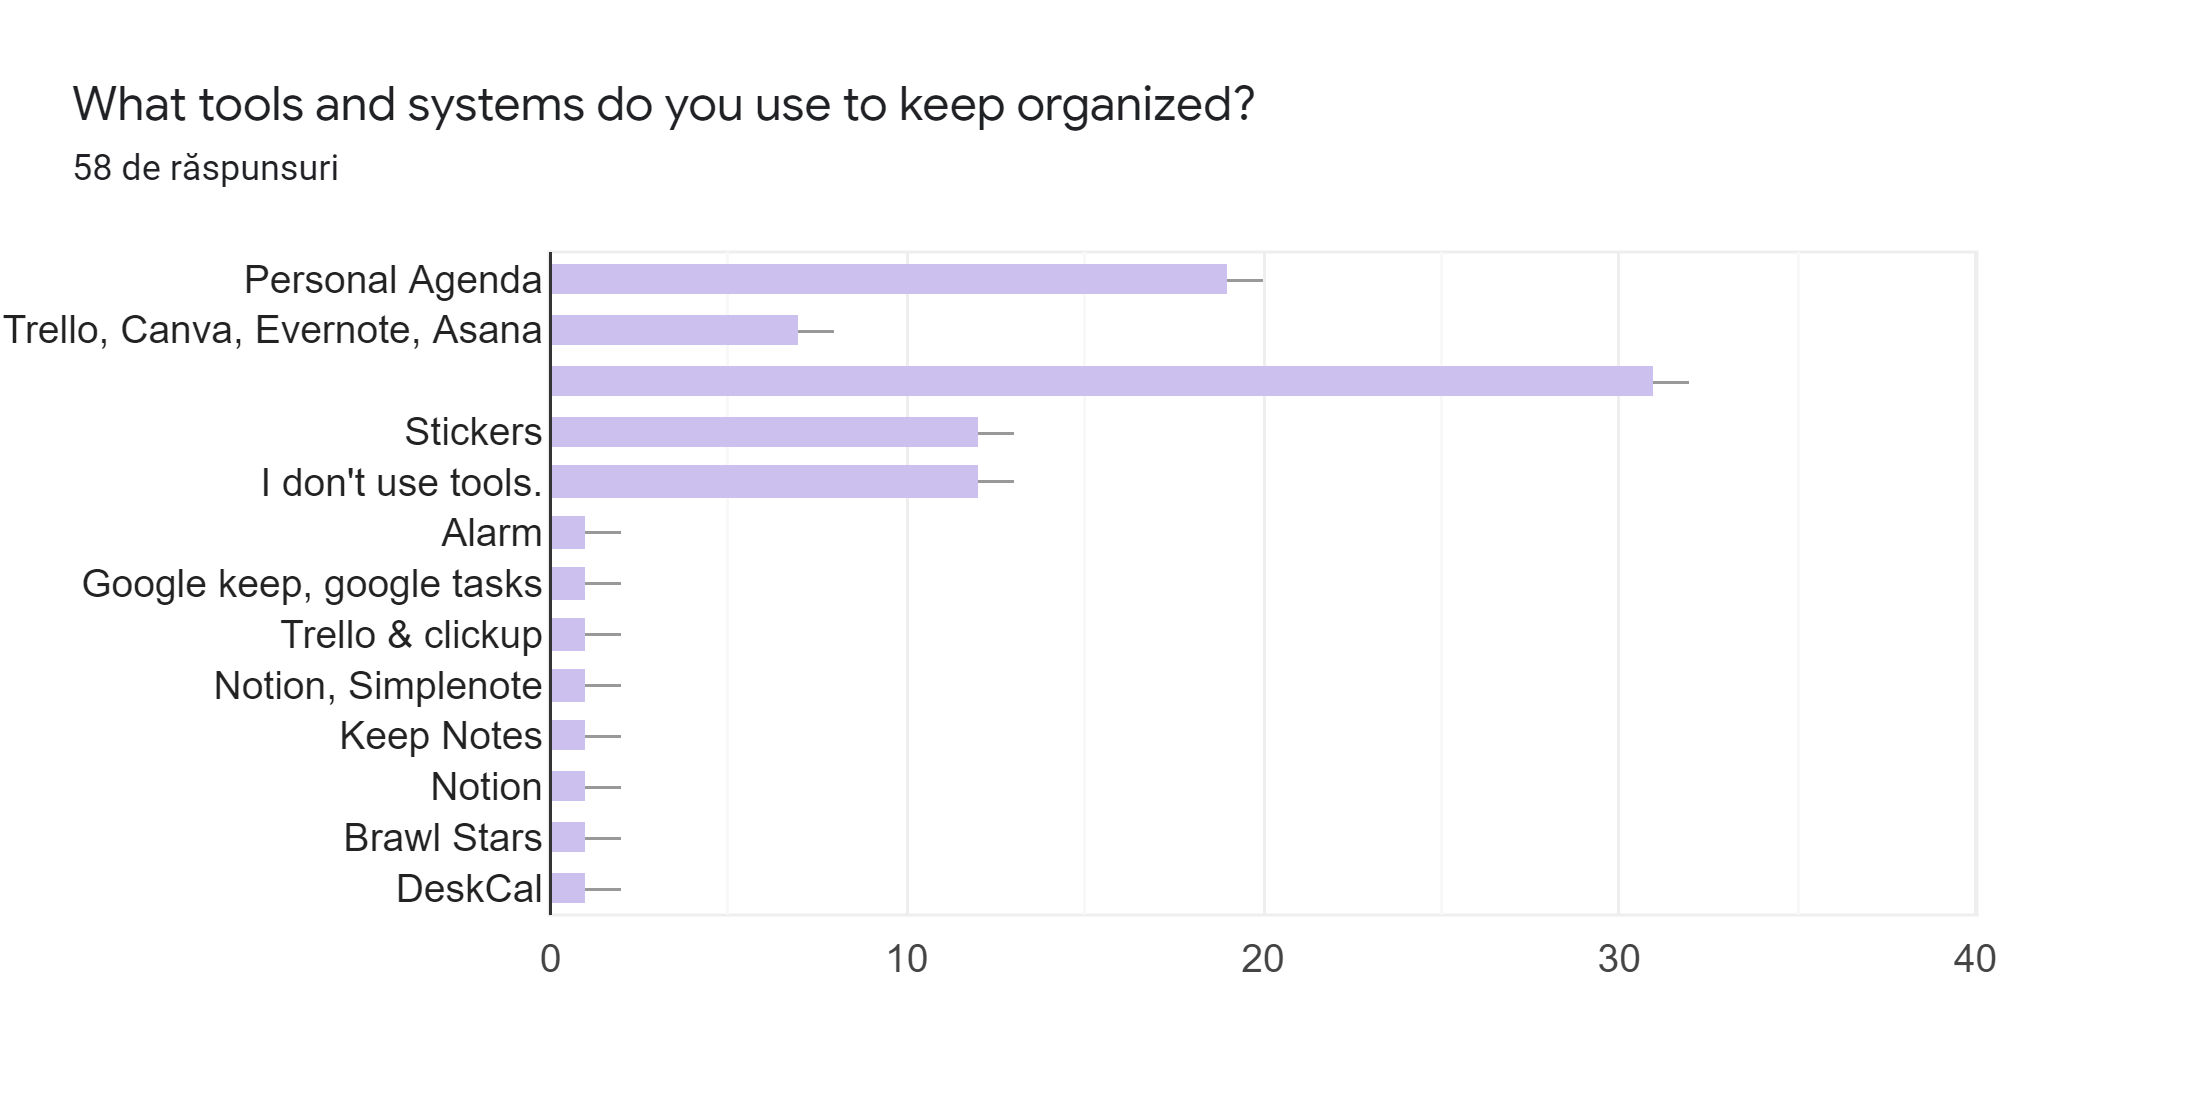
\includegraphics[width=\textwidth]{CustomerValidation3}
\par 31 humans use Google Calendar, Outlook Calendar, Todoist. This means that people like to view their task, activities, meetings in a calendar way of displaying. The second place take agendas with 19 votes. This means that even that we live in very digitalized world people choose to use the paper-based type of managing their activities and thoughts.
\par
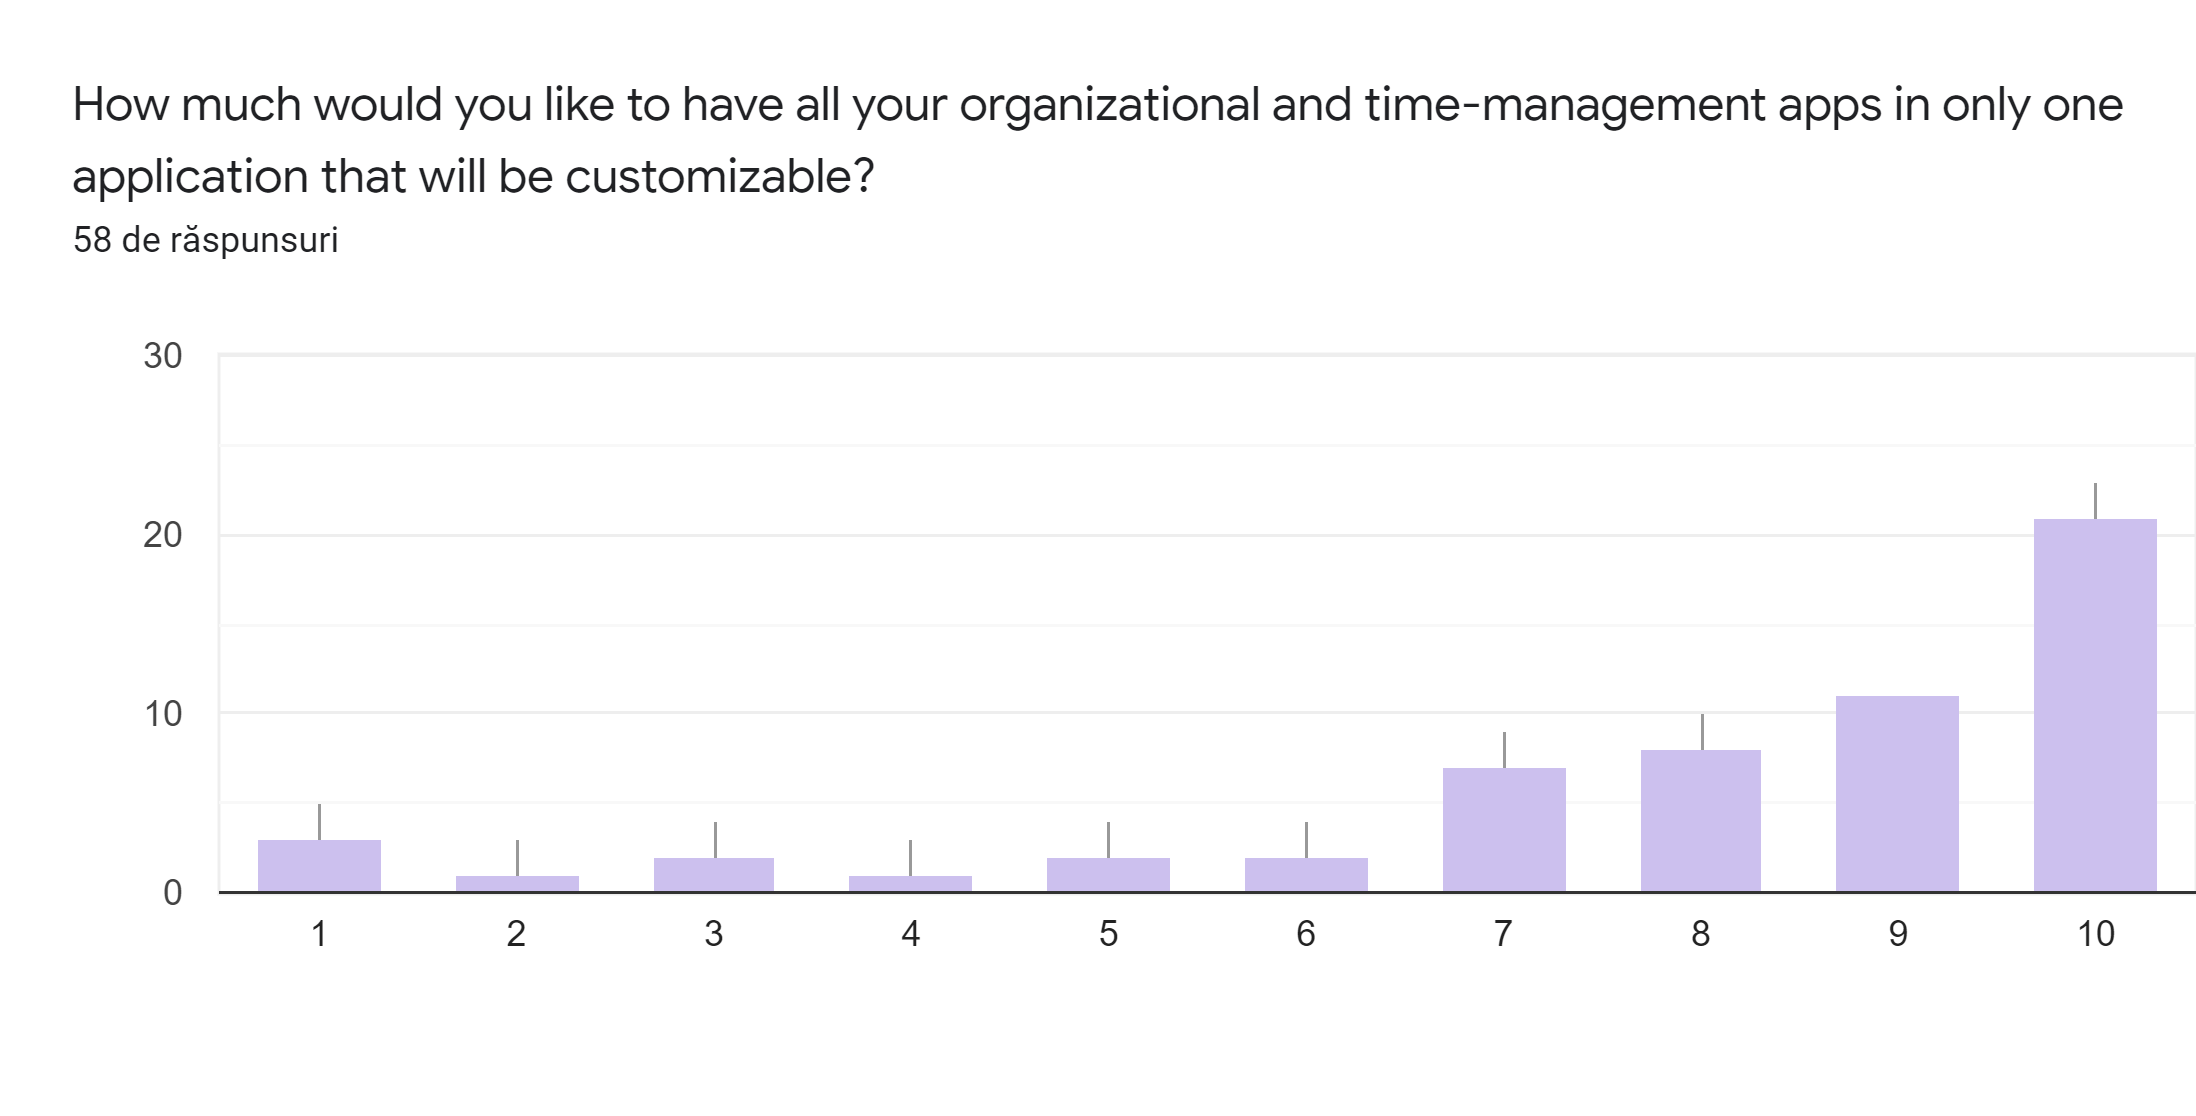
\includegraphics[width=\textwidth]{CustomerValidation4}
\par 30 assume that their desire of having an organizational and time-management app that will be customizable and will be integrated with other calendar apps is graded with 9 or 10. This is more than a half of total number of people took part and this means that the interest in such an application is highly shown. This means that developing such a concept has the right to be in production.
\par
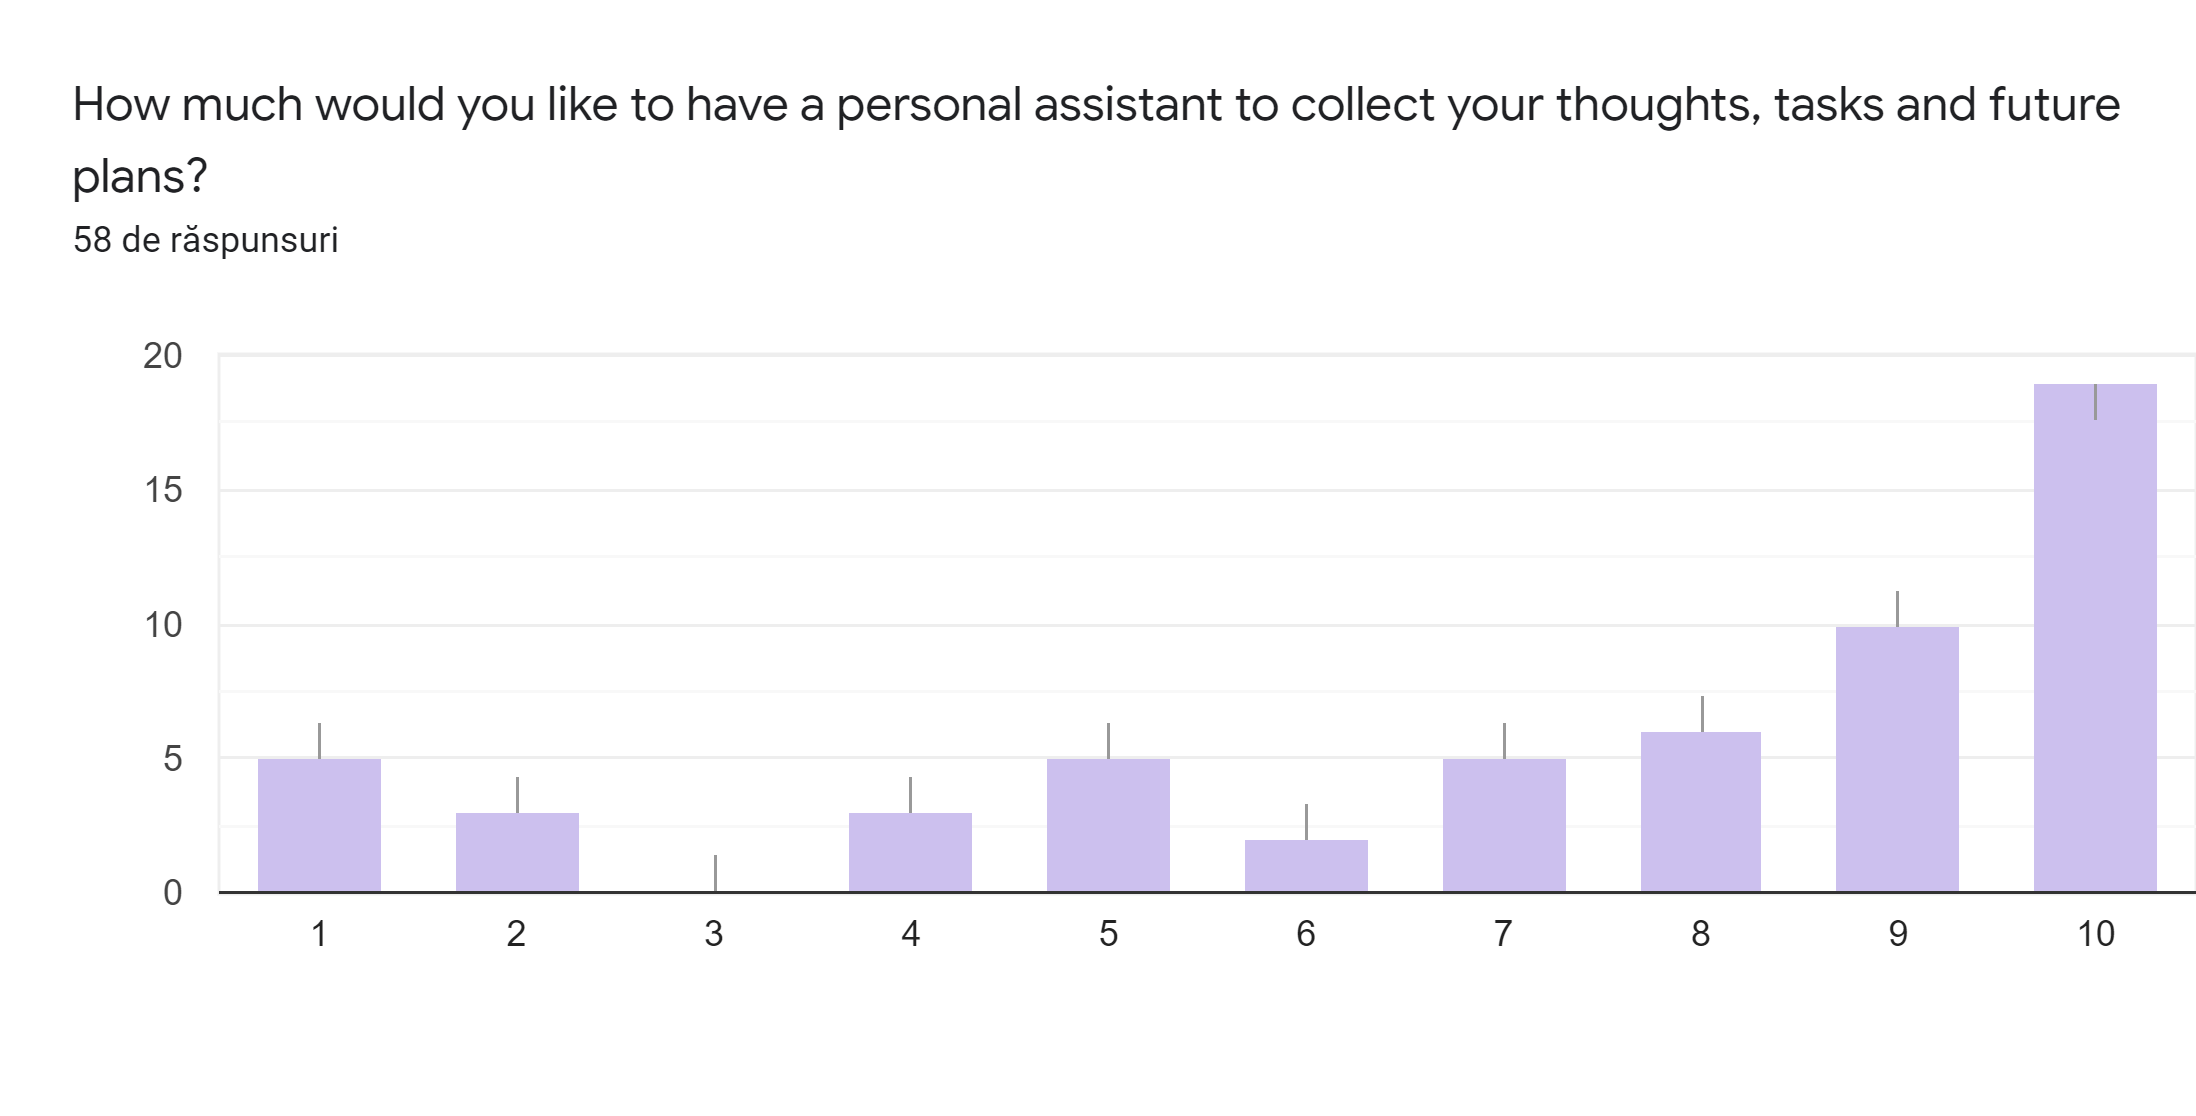
\includegraphics[width=\textwidth]{CustomerValidation5}
\par 29 people shown surely that they want to have a personal assistant to collect their thoughts, tasks and plans. It can be understood that future customers are highly interested in both of our main advantages over competitors.

\subsection{Competition}
\par 
\begin{enumerate}
	\begin{figure}[h]
		\centering
		
\includegraphics[width=0.5\textwidth ]{Google_Calendar.max-1100x1100}
		\caption{Google Calendar Logo}	
	\end{figure}

	\item 	Google calendar is not the most intuitive app of using tasks and schedules it has a lot of special conditions to get the desired result also it is consisting in a big platform google where cam communicate with other google application so it easy to work  
	
	We have made a research and found out the common problems of Google Calendar: 
	
	If the calendar doesn't belong to you and hasn't been shared with you, Google will not provide the Summary or Description fields. The solution is simple, have the owner share the calendar with you (even if it is public)! 
	
	Repeated events in Google Calendar aren't supported with the "New Event" trigger in Zapier. A repeated event would cause an infinite amount of Tasks to occur since repeated events last forever. However, repeated events can be used with the "Event Starts" trigger. 
	
	All-day events in Google Calendar end at midnight on the last day, so they're exclusive of the end date. For example, an event created via Zapier for August 10 - August 15 will appear to span August 10 - August 14 in the calendar UI, because the event will end at 12:00:00 on August 15. 
	
	To fix this, you can either update your trigger data so that it lasts for an extra day, or you can modify the end date in your Zap directly by adjusting the date/time to include +1d. This will cause the event to last for an extra day. 
	
	If you're using the "Quick Add Event" action instead of the "Create Detailed Event" action, there are some specific guidelines you'll want to follow to make sure that Google Calendar can interpret the date and time correctly. 
	
	If you set the start date time and end date time to the exact same time it's possible that you might not see the event in Google Calendar when you are looking at the calendar in some views. If you click on agenda view in Google Calendar you will see the event show up. Google Calendar doesn't show events with a length on 0 minutes in some of their other views. 
	
	Unfortunately, Google changes the ID of events on their auto-generated calendar in a way that causes the same event to trigger multiple times. We don't recommend building zaps on Google generated calendars because of this. 
	
	Google is finicky in recognizing dates/times when using Quick Add, and you'll have to include the information in a format that Google can recognize. Specifically,: 
	
	Event details need to follow the order: what, where, when. Events created with the details in a different order may not be parsed correctly. 
	
	If you enter an event with no date, it will be added at the next available time in the future 
	
	If you don't enter a start time, an all-day event will show up 
	
	If you don't enter an end time, an hour-long event will show up 
	
	Unfortunately the Quick Add Event action doesn't allow you to invite users to an event, it'll just add it to their calendar. If you'd like to send the user an invitation that they can accept/reject, you'll want to use the Create Detailed Event action instead. 
	
	

		\begin{figure}[h]
		\centering
		
\includegraphics[width=0.5\textwidth ]{SuperSaaS_Word}
		\caption{SuperSaaS Logo}
	\end{figure}
	
	\item SuperSaaS is good at creating group schedule, but because of the design of the site is hard to understand what happens, saves the situation the support and tutorials page, it supports the work with forms directly when accessing the schedule which is very efficient in scope to get additional information but it faces issues when it comes to sharing and working across multiple time zones
	


		\begin{figure}[h]
		\centering
		\includegraphics[width=0.5\textwidth ]{1200px-Microsoft_Office_Outlook_(2018–present).svg}
		\caption{Outlook Logo}
	\end{figure}

	\item Outlook to get all the possibilities of the calendar you need to pay, is free for students and have many integrated applications which can communicate direct whit each other that increase productivity it is a combination of calendar and email it is very easy to share about events and set tasks and reminders for groups or selected people but because outlook is a system of big amount of interconnected tools is very hard to understand at start also there are problems with meeting approving, storage security and automatic secure control of account.  
	
	
	

	\begin{figure}[h]
		\centering
		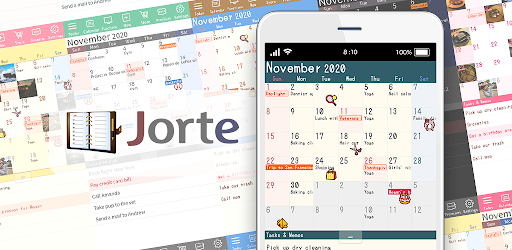
\includegraphics[width=0.5\textwidth ]{Jorte_Calendar}
		\caption{Jorte Calendar Logo}
	\end{figure}

	\item Jorte Calendar theme changing, can use free but to get the chance to change the appearance of the calendar you need to pay subscription but it faces problems with synchronization between other calendars and problems with time zones calibration.
	
		
    \begin{figure}[h]
    	\centering
    	
\includegraphics[width=0.5\textwidth ]{Calendly}
    	\caption{Calendly Logo}
    \end{figure}

	\item Calendly it is app which works very good with establishing new meetings and events because it gave you to choose the rules that all participants can choose between the permission you establish it is time zone but the free users are limited to 1 calendar and basic functions which do not let user to feel the power of this app also even if is paid version it is facing a lot of problems with reminding the meetings and problem with booking system and there is no proper customer service.
	
	\begin{figure}[h]
		\centering
		
\includegraphics[width=0.5\textwidth ]{clockwise-logo}
		\caption{Clockwise Logo}
	\end{figure}
		
	\item Clockwise Protecting travel time, Automatic color code, personal and work calendars in sync, resolving meeting conflicts, handling different time zones, and always saving time for lunch. 
	
	\begin{figure}[h]
		\centering
		
\includegraphics[width=0.5\textwidth ]{reclaimai-logo}
		\caption{Reclaim AI Logo}
	\end{figure}	
	
	\item Reclaimai, flexible scheduling finds and defends time on calendar, makes and schedule automatic regularly routine that can be chosen from a customizable list  
	
		
	
\end{enumerate}				

\clearpage